\documentclass[10pt]{article}
\usepackage{titling}
\usepackage[margin=0.75in]{geometry}
\usepackage{graphicx}
\graphicspath{ {images/}}
\title{Requirements Document}
\author{
	Dylan Davis, Trevor Hammock, Alex Schultz \\
	Oregon State University\\
	Corvallis, Oregon
}
\date{\today}

\begin{document}
\begin{titlingpage}
\maketitle

\begin{abstract}

This document describes the requirements for completion of the HP data compression capstone project. Because this is a research based project, the requirements are given as research milestones describing when the group plans to start and complete the different areas of research that will be covered over the course of the year. Also within this document are descriptions of the purpose and scope of the project, definitions of relevant terms, and an overview of the various pieces of software that will be used to run and analyze experiments. References to important sources of information pertaining to the project are provided as well as stretch goals to be explored if the primary goals of the project are fulfilled. 

\end{abstract}
\end{titlingpage}


\tableofcontents
\clearpage


\section{Introduction}
\subsection{Purpose}

PageWide Web Press, a printing division within HP, produces and supports industrial digital web presses. All of the web presses currently deployed  in the market generate product data, which the PageWide Web Press team receives on a daily basis. The data is eventually stored into a Oracle Database and is used to perform business analytics and resolve issues with the web presses.

However, this data is currently creating some issues for the division. On average, the division receives around 350GB of product data per day, which generates Database tables with over billions of rows. This massive influx of data has stressed the division's storage and performance capabilities of their current hardware. The stress on the hardware significantly increases the amount time it takes to process and analyze that data, and the division wants to find a more efficient data storage solution. Furthermore, the amount of data that is received everyday has slowly been increasing over time. The current rate of 350GB of data per day could turn into 450 to 500 GB of data very quickly.

If nothing is done about the data collection process, the division may need make a costly investment into better hardware that can meet their growing storage and performance needs. Alternatively, they may have to invest into big data software platforms, like Hadoop, that are more optimized and scalable for their given workloads. This project will address the aforementioned issues by using system enabled compression to reduce the amount of physical space that the data occupies.


\subsection{Scope}

The current scope of the project is to investigate various Oracle database compression options and use them to implement a solution for PageWide Web Press' storage crisis. The solution will not alter or restructure the data itself, but rather change how the Database system stores said data into the physical storage medium. It is not a requirement to actively look into or investigate query performance options for this solution (like Oracle's in-memory compression for example [1]).

Essentially, the goal of this project is to address the division's data issues by using compression to reduce the amount of space that the data occupies. If implemented properly, compression should help delay a costly hardware/software upgrade for their storage needs and hopefully improve the query performance for their database system.


\subsection{Definitions, acronyms, and abbreviations}

\begin{center}
    \begin{tabular}{ | l | p{11cm} |}
    \hline
    \textbf{Term} & \textbf{Definition}  \\ \hline
    Block & The smallest unit of storage in an Oracle Database \\ \hline
    Central Processing Unit (CPU) & Physical processor that executes instructions  \\ \hline
    Command Line (CLI) & A application which provides a means of interacting with a computer program by entering lines of \\ \hline
    Database & Software that stores data in an organized fashion \\ \hline
    Database Administrator (DBA) & A person responsible for the efficiency of a system's database including security, scalability, reliability, and performance \\ \hline
    Hadoop & Software framework optimized and designed for processing big data \\ \hline
    Hewlett-Packard (HP) & Multinational IT company that is infamous for their printing products \\ \hline
    IDE (Integrated Development Environment) & A software application that provides comprehensive facilities to computer programmers for software development \\ \hline
    Input/Output (I/O) & Typically associated with the rate of how data is read or written to a physical storage medium \\ \hline
    Oracle & Multinational IT company that specializes in enterprise solutions such as Database software and cloud systems \\ \hline
    Oracle Database & A relational database system that is produced and supported by Oracle \\ \hline
    Oracle Linux & Distribution of Linux that is maintained by Oracle. It is optimized platform for many of their products, such as Oracle Database \\ \hline
    PageWide Web Press & A printing division within HP that develops and supports HP's industrial digital web presses \\ \hline
    Query & A request that processes and/or returns data from within a database \\ \hline
    Oracle Recovery Manager (RMAN) & An Oracle product that is used to backup and recover Oracle Databases \\ \hline
    Secure Shell (SSH) &  Cryptographic network protocol for operating network services securely over an unsecured network. \\ \hline
    Stakeholder & Someone who is not a DBA or developer but is otherwise involved \\ \hline
    \end{tabular}
\end{center}



\subsection{References}

\begin{flushleft}
T. Chien and S. Wertheimer, “Recovery Manager (RMAN) Performance Tuning Best Practices,” Jun-2011. [Online]. Available: http://www.oracle.com/technetwork/database/focus-areas/availability/rman-perf-tuning-bp-452204.pdf. [Accessed: 03-Nov-2017] \hfill \break

A. Dadhich, K. Patel, F. Khan, and S. Pamu, “Advanced Network Compression,” Dec-2013. [Online]. Available: http://www.oracle.com/technetwork/database/enterprise-edition/advancednetworkcompression-2141325.pdf. [Accessed: 03-Nov-2017] \hfill \break

“Oracle Advanced Compression with Oracle Database 12 c Release 2,” Sep-2017. [Online]. Available: http://www.oracle.com/technetwork/database/options/compression/advanced-compression-wp-12c-1896128.pdf. [Accessed: 03-Nov-2017] \hfill \break

A. Rivenes, M. Colgan, and V. Marwah, “Oracle Database In - Memory with Oracle Database 12c Release 2 Technical Overview,” Aug-2017. [Online]. Available: http://www.oracle.com/technetwork/database/in-memory/overview/twp-oracle-database-in-memory-2245633.pdf. [Accessed: 03-Nov-2017] \hfill \break
\end{flushleft}


\subsection{Overview}

The second section of this requirements document gives an overview of how the project interacts with other systems, intended functions, characteristics, given constraints, and assumptions. This section is written for the individual stakeholders and examines the project at a much higher level. The third section of this requirements document details the individual requirements that will be implemented. This section possess a lot of technical aspects/terminology and is intended for the implementers for this project. Together these sections form a comprehensive overview for this document.


\section{Overall Description}
\subsection{Product perspective}

This activity is not a standalone piece of software but rather it runs on top of a pre-existing system. This project will emulate a Database environment that closely matches the client. The environment will based on a Oracle Linux distribution which will host an Oracle Database instance, and it will serve as the testing grounds for the project's tests and analysis. This will allow the individuals working on this project to make conclusions about Oracle's compression for their Databases.


\subsubsection{System Interfaces}

The primary system interface will be the operating system for Oracle Databases, Oracle Linux 7. The Databases that we will create and test will run on this distribution of Linux. For system analysis, system calls will be made to gather any relevant information/data.


\subsubsection{User Interfaces}

The user interfaces will be the Linux command line and SQL Developer IDE. The command line and the IDE will both be used to run queries on the Database to interact with it. Additionally the command line will be used to alter system settings or parameters, such as starting up the Database instance.


\subsubsection{Hardware Interfaces}

No hardware interfaces are involved; the task is software based, and a virtual machine will be used to emulate the client's system. 


\subsubsection{Software Interfaces}

Oracle 12.2 Database instance on top of Oracle Linux 7 environment. The following system software is required for this project:

\begin{itemize}
	\item Oracle Linux 7
    \begin{itemize}
    	\item Mnemonic: OL7
        \item Version: 7.4
        \item Source: Oracle
    \end{itemize}

    \item Oracle Database 12c Enterprise Edition
    \begin{itemize}
    	\item Mnemonic: 12c
        \item Version: 12.2.0.1.0
        \item Source: Oracle
    \end{itemize}

	\item Oracle SQL Developer
    \begin{itemize}
    	\item Mnemonic: N/A
        \item Version: 17.3.0
        \item Source: Oracle
    \end{itemize}

	\item Linux Command Line Interface
    \begin{itemize}
    	\item Mnemonic: CLI
        \item Version: 3.10.0
        \item Source: Linux
    \end{itemize}
\end{itemize}

\subsubsection{Communications}

We will be remotely connecting and running commands/scripts to the emulated system. The network configuration will be done through the routine Oracle Database hosting procedures. Once the network configuration is setup, SQL Developer and SSH terminals will be used to remotely interact with the system.


\subsubsection{Memory Constraints}

The Database instance and all of the tables containing our data will need to fit within the allocated space for the virtual machine (60GB; 4GB RAM).


\subsubsection{Operations}

There will be multiple modes of operations, including sys level access and basic user access. Sys access will be used to manage the underlying system such as modifying how the data in the Database gets stored. User access will be used for generating and testing the data. Most of the periods of operation will be run in the background unless it is explicitly forced to run. Should time allow, and the backup/recovery options are explored, then explicit backups will be made for testing purposes.


\subsubsection{Site Adaptation Requirements}

There are no site specific requirements for this project.


\subsection{Product functions}

There are no explicit functions for this project. 


\subsection{User characteristics}

Users interacting with the system and performing the analyses will be Database Administrators (DBA's) that manage Databases for their systems or product stacks. The users should be proficient in SQL, Oracle Database specifics, and Unix/Linux system administration.


\subsection{Constraints}
Only compression options available in Oracle Database 12.2 will be considered. System characteristics and properties will also be analyzed; for example, the effect block size has on the varying compression algorithms. Compression options with stricter licensing or hardware dependencies will be ignored; in other words, if it's not free, it's not a viable option. The data, and how it is structured, will be left intact; however, data stored in the physical storage medium will change. Compression options that show little to no benefits will be ignored in the final implementation.
Data properties and characteristics will also be examined, which will include:
		\begin{itemize}
			\item How the columns are ordered
			\item The cardinality
			\item Repetition within the datasets
		\end{itemize}


\subsection{Assumptions and dependencies}
It is assumed that all of Databases used in this project will be installed on a distribution of Oracle Linux 7. Additionally, Oracle Databases used in this project will be version 12.2, and the system performing the benchmarks for this project can record system statistics, such as CPU usage, within a reasonable time resolution.

\subsection{Apportioning of requirements}

If time permits, the following stretch goals may be investigated and potentially implemented:
\begin{itemize}
	\item Enabling Oracle's new Network Compression [2] and see the effect it has network bandwidth.
	\item Researching and/or playing with Oracle's Advanced Index Compression [3] to investigate additional space/performance savings.
	\item Oracle's Backup Compression (RMAN) [4] to address future storage issues with their regularly scheduled backups.
\end{itemize}

\section{Requirements}

All tests and analyses will be performed on systems/data that mirror PageWide Web Press' current environment. The members conducting this project will learn about and reverse engineer data blocks in Oracle to understand how the data gets stored. Oracle compression algorithms will be tested and reverse engineered (to the best that can be inferred) to understand how it interacts with a sample set of data. Once the background research is complete, the project facilitators will then design a set of experiments to prove/test the findings they found during the research phase. Experiments include creating and using a set of scripts that will track critical system information such as CPU, I/O, and/or Memory usage. Once all of the data from the experiments is collected, it will be compiled into a white paper that will summarize the research and findings. Finally, the white paper will be presented at an Oracle Database conference in the Spring entitled Hotsos. The remainder of the project will be reserved for design and possibly integrating a solution into PageWide Web Press's current environment.

Gantt Chart outlining the tasks and tentative due dates: \\
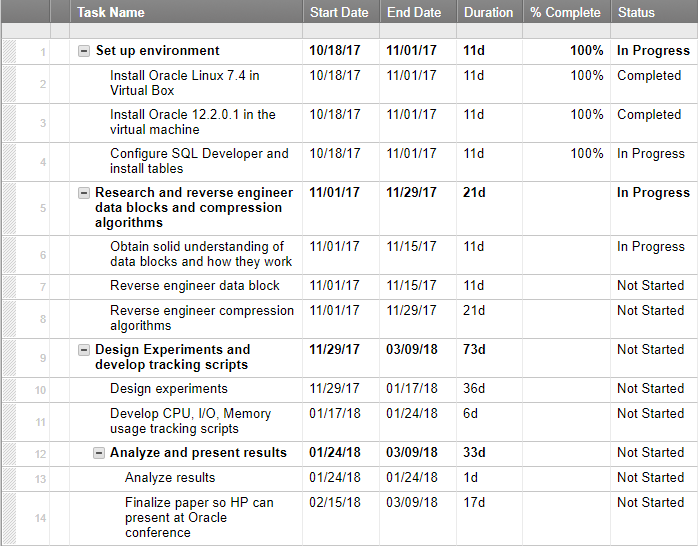
\includegraphics{gantt.png}


\end{document}